\section{Na-D Linie}
\subsection{Korrekturfaktor des Motors M2}
Die Schwebungsfrequenz der beiden Natrium-D Linien lässt sich wie folgt berechnen:
\begin{equation}
    f_{sch.}=\left|f_{D2}-f_{D1}\right|
\end{equation}
Die Frequenzen der beiden Linien ($f_{D2}$ und $f_{D1}$) lassen sich mithilfe den Literaturwerten für die beiden Wellenlängen der Linien berechnen.\\
Für die erste Natrium-D Linie folgt: $\lambda_{D1}=589,593\,\text{nm}$\\
Und für die zweite D-Linie folgt: $\lambda_{D2}=588,996\,\text{nm}$\\
Diese müssen noch in Frequenzen umgerechnet werden:
\begin{equation}
    f=\frac{c}{\lambda}
\end{equation}
Somit folgt für die Frequenzen der Natrium-D Linien:
\begin{align}
    f_{D1}&=5,083\cdot10^{14}\,\text{Hz}\\
    f_{D2}&=5,090\cdot10^{14}\,\text{Hz}
\end{align}
Und die Schwebungsfrequenz:
\begin{equation}
    f_{sch.}=5,154\cdot10^{11}\,\text{Hz}
\end{equation}
Für die theoretische Schwebungswellenlänge folgt:
\begin{equation}
    \lambda_{{sch.}_{theo.}}=\frac{c}{f_{sch.}}=0,5817\,\text{mm}
\end{equation}\newpage
Um den Korrekturfaktor des Motors $M2$ zu bestimmen, werden die Peaks der Einhüllende bestimmt:
\begin{figure}[h]
    \centering\scalebox{0.8}{% GNUPLOT: LaTeX picture with Postscript
\begingroup
  % Encoding inside the plot.  In the header of your document, this encoding
  % should to defined, e.g., by using
  % \usepackage[cp1252,<other encodings>]{inputenc}
  \inputencoding{cp1252}%
  \makeatletter
  \providecommand\color[2][]{%
    \GenericError{(gnuplot) \space\space\space\@spaces}{%
      Package color not loaded in conjunction with
      terminal option `colourtext'%
    }{See the gnuplot documentation for explanation.%
    }{Either use 'blacktext' in gnuplot or load the package
      color.sty in LaTeX.}%
    \renewcommand\color[2][]{}%
  }%
  \providecommand\includegraphics[2][]{%
    \GenericError{(gnuplot) \space\space\space\@spaces}{%
      Package graphicx or graphics not loaded%
    }{See the gnuplot documentation for explanation.%
    }{The gnuplot epslatex terminal needs graphicx.sty or graphics.sty.}%
    \renewcommand\includegraphics[2][]{}%
  }%
  \providecommand\rotatebox[2]{#2}%
  \@ifundefined{ifGPcolor}{%
    \newif\ifGPcolor
    \GPcolorfalse
  }{}%
  \@ifundefined{ifGPblacktext}{%
    \newif\ifGPblacktext
    \GPblacktexttrue
  }{}%
  % define a \g@addto@macro without @ in the name:
  \let\gplgaddtomacro\g@addto@macro
  % define empty templates for all commands taking text:
  \gdef\gplbacktext{}%
  \gdef\gplfronttext{}%
  \makeatother
  \ifGPblacktext
    % no textcolor at all
    \def\colorrgb#1{}%
    \def\colorgray#1{}%
  \else
    % gray or color?
    \ifGPcolor
      \def\colorrgb#1{\color[rgb]{#1}}%
      \def\colorgray#1{\color[gray]{#1}}%
      \expandafter\def\csname LTw\endcsname{\color{white}}%
      \expandafter\def\csname LTb\endcsname{\color{black}}%
      \expandafter\def\csname LTa\endcsname{\color{black}}%
      \expandafter\def\csname LT0\endcsname{\color[rgb]{1,0,0}}%
      \expandafter\def\csname LT1\endcsname{\color[rgb]{0,1,0}}%
      \expandafter\def\csname LT2\endcsname{\color[rgb]{0,0,1}}%
      \expandafter\def\csname LT3\endcsname{\color[rgb]{1,0,1}}%
      \expandafter\def\csname LT4\endcsname{\color[rgb]{0,1,1}}%
      \expandafter\def\csname LT5\endcsname{\color[rgb]{1,1,0}}%
      \expandafter\def\csname LT6\endcsname{\color[rgb]{0,0,0}}%
      \expandafter\def\csname LT7\endcsname{\color[rgb]{1,0.3,0}}%
      \expandafter\def\csname LT8\endcsname{\color[rgb]{0.5,0.5,0.5}}%
    \else
      % gray
      \def\colorrgb#1{\color{black}}%
      \def\colorgray#1{\color[gray]{#1}}%
      \expandafter\def\csname LTw\endcsname{\color{white}}%
      \expandafter\def\csname LTb\endcsname{\color{black}}%
      \expandafter\def\csname LTa\endcsname{\color{black}}%
      \expandafter\def\csname LT0\endcsname{\color{black}}%
      \expandafter\def\csname LT1\endcsname{\color{black}}%
      \expandafter\def\csname LT2\endcsname{\color{black}}%
      \expandafter\def\csname LT3\endcsname{\color{black}}%
      \expandafter\def\csname LT4\endcsname{\color{black}}%
      \expandafter\def\csname LT5\endcsname{\color{black}}%
      \expandafter\def\csname LT6\endcsname{\color{black}}%
      \expandafter\def\csname LT7\endcsname{\color{black}}%
      \expandafter\def\csname LT8\endcsname{\color{black}}%
    \fi
  \fi
    \setlength{\unitlength}{0.0500bp}%
    \ifx\gptboxheight\undefined%
      \newlength{\gptboxheight}%
      \newlength{\gptboxwidth}%
      \newsavebox{\gptboxtext}%
    \fi%
    \setlength{\fboxrule}{0.5pt}%
    \setlength{\fboxsep}{1pt}%
\begin{picture}(7200.00,5040.00)%
    \gplgaddtomacro\gplbacktext{%
      \csname LTb\endcsname%%
      \put(946,704){\makebox(0,0)[r]{\strut{}$0.02$}}%
      \put(946,1116){\makebox(0,0)[r]{\strut{}$0.03$}}%
      \put(946,1527){\makebox(0,0)[r]{\strut{}$0.04$}}%
      \put(946,1939){\makebox(0,0)[r]{\strut{}$0.05$}}%
      \put(946,2350){\makebox(0,0)[r]{\strut{}$0.06$}}%
      \put(946,2761){\makebox(0,0)[r]{\strut{}$0.07$}}%
      \put(946,3173){\makebox(0,0)[r]{\strut{}$0.08$}}%
      \put(946,3585){\makebox(0,0)[r]{\strut{}$0.09$}}%
      \put(946,3996){\makebox(0,0)[r]{\strut{}$0.1$}}%
      \put(946,4408){\makebox(0,0)[r]{\strut{}$0.11$}}%
      \put(946,4819){\makebox(0,0)[r]{\strut{}$0.12$}}%
      \put(1078,484){\makebox(0,0){\strut{}$30$}}%
      \put(1588,484){\makebox(0,0){\strut{}$32$}}%
      \put(2099,484){\makebox(0,0){\strut{}$34$}}%
      \put(2609,484){\makebox(0,0){\strut{}$36$}}%
      \put(3120,484){\makebox(0,0){\strut{}$38$}}%
      \put(3630,484){\makebox(0,0){\strut{}$40$}}%
      \put(4141,484){\makebox(0,0){\strut{}$42$}}%
      \put(4651,484){\makebox(0,0){\strut{}$44$}}%
      \put(5162,484){\makebox(0,0){\strut{}$46$}}%
      \put(5672,484){\makebox(0,0){\strut{}$48$}}%
      \put(6183,484){\makebox(0,0){\strut{}$50$}}%
      \put(6693,484){\makebox(0,0){\strut{}$52$}}%
    }%
    \gplgaddtomacro\gplfronttext{%
      \csname LTb\endcsname%%
      \put(209,2761){\rotatebox{-270}{\makebox(0,0){\strut{}Intensit\"at [V]}}}%
      \csname LTb\endcsname%%
      \put(6748,2761){\rotatebox{-270}{\makebox(0,0){\strut{}}}}%
      \csname LTb\endcsname%%
      \put(3885,154){\makebox(0,0){\strut{}Motorposition [mm]}}%
      \csname LTb\endcsname%%
      \put(3885,4819){\makebox(0,0){\strut{}}}%
      \csname LTb\endcsname%%
      \put(132,-110){\makebox(0,0)[l]{\strut{}}}%
      \csname LTb\endcsname%%
      \put(5706,4646){\makebox(0,0)[r]{\strut{}Einh\"ullende}}%
      \csname LTb\endcsname%%
      \put(5706,4426){\makebox(0,0)[r]{\strut{}Peaks}}%
    }%
    \gplbacktext
    \put(0,0){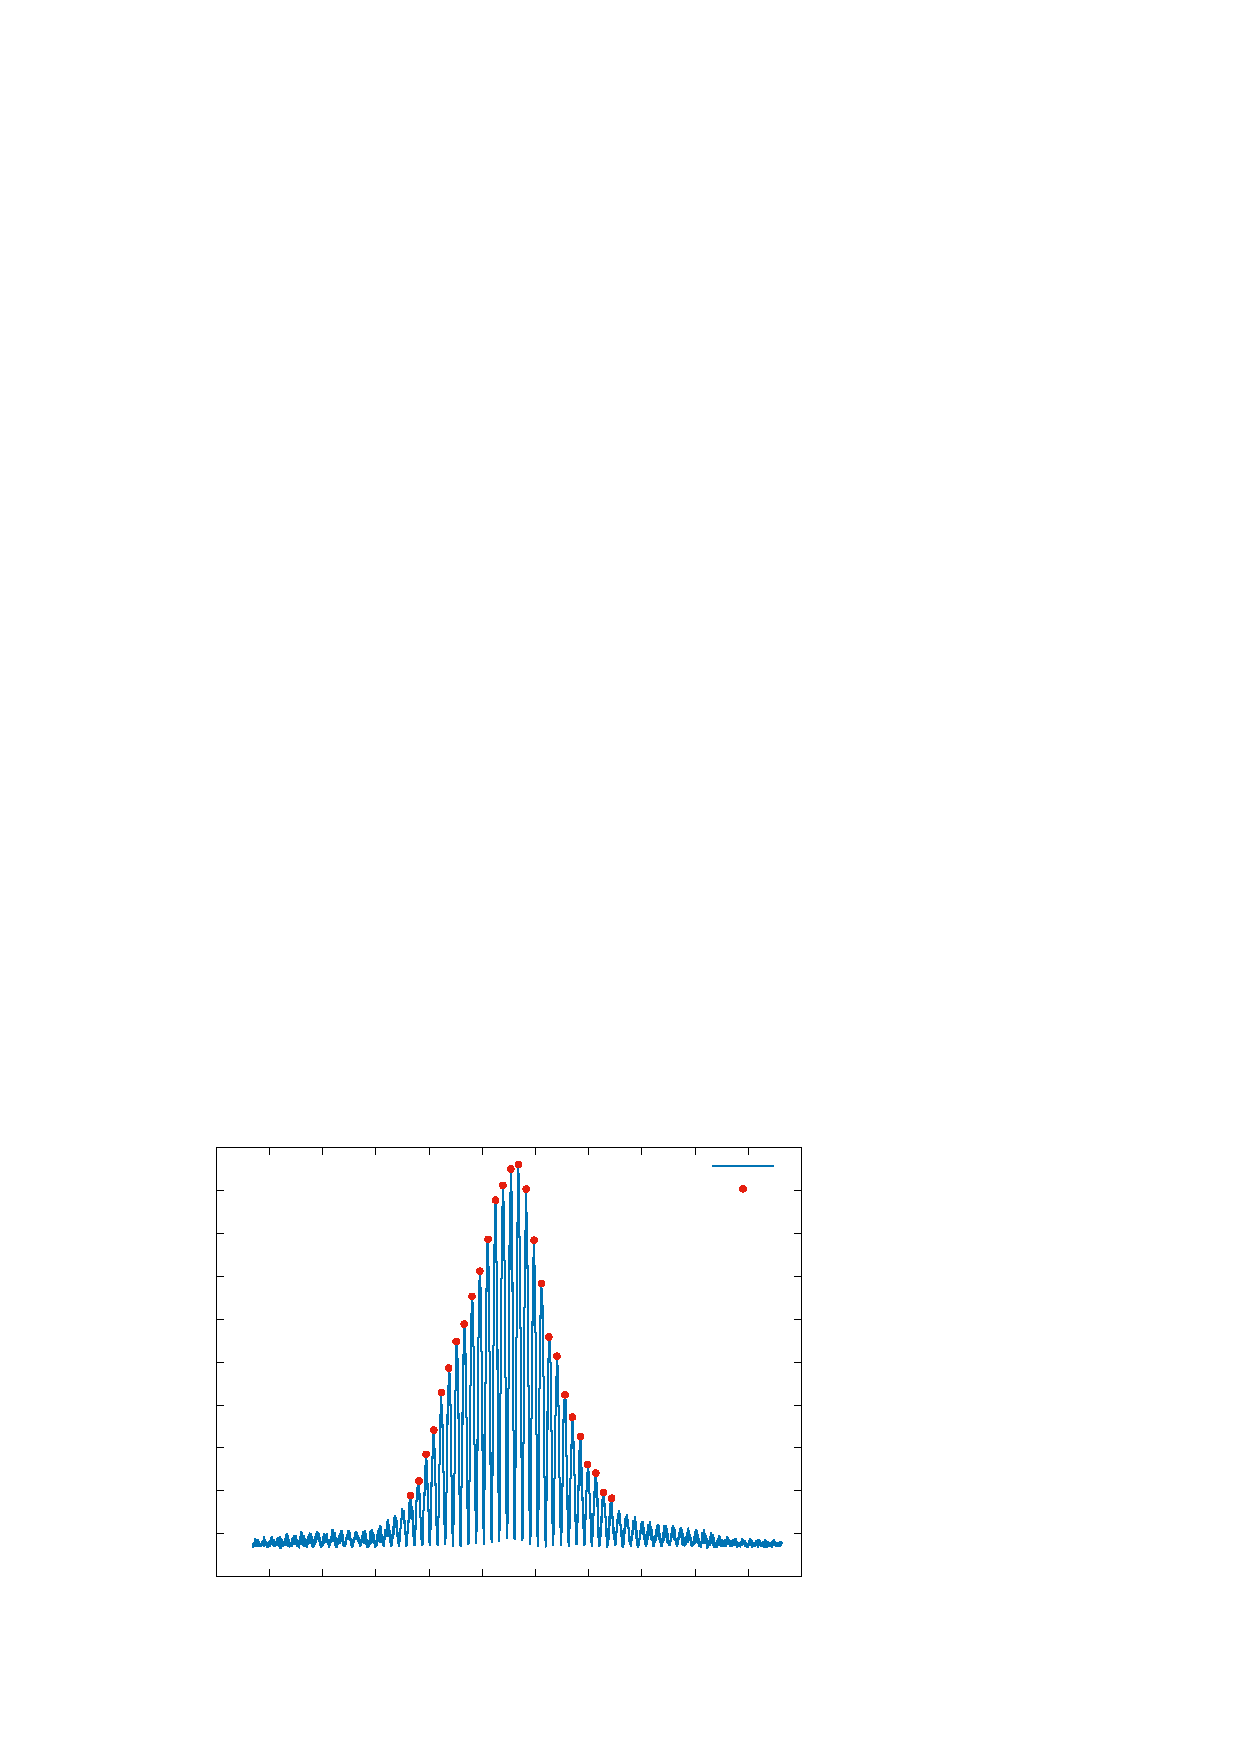
\includegraphics[width={360.00bp},height={252.00bp}]{Dominik/einhuellende_na}}%
    \gplfronttext
  \end{picture}%
\endgroup
}
    \caption{Einhüllende der Na-D Linie mit den eingezeichneten Peaks.}
\end{figure}\\
Der Abstand zwischen zwei Peaks wurde für alle Werte bestimmt und anschließend gemittelt.
Dann erhalten wir den mittleren Abstand:
\begin{equation}
    \bar{p}=\left(0,2913\pm0,0002\right)\,\text{mm}
\end{equation}
Da das Licht die doppelte Weglänge zurücklegt, folgt für die gemessene Wellenlänge der Schwebung:
\begin{equation}
    \lambda_{{sch.}_{mess}}=\left(0,5826\pm0,0004\right)\,\text{mm}
\end{equation}
Der Korrekturfaktor des Motors $M2$ bestimmt sich nun, indem man das Verhältnis aus gemessener und theoretischer Schwebungswellenlänge berechnet:
\begin{equation}
    \beta=\frac{\lambda_{{sch.}_{theo.}}}{\lambda_{{sch.}_{mess}}}
\end{equation}
Somit folgt für den Korrekturfaktor:
\begin{equation}
    \beta=0,998\pm0,001
\end{equation}
Mit diesem kann man die experimentell gemessenen Wegstrecken in die eigentlich gefahrenen Wegstrecken umrechnen:
\begin{equation}
    \lambda_{{sch.}_{theo.}}=\beta\cdot\lambda_{{sch.}_{mess}}
\end{equation}
\subsection{Wellenlänge, Kohärenzlänge und Linienbreite der Linie}
\subsubsection{Wellenlänge bestimmen}
Um die Wellenlänge der Natriumdampflampe zu bestimmen, werden die Peaks des aufgenommenen Spektrums gezählt ($n_{Na}$).
Diese werden anschließend durch die Anzahl der Peaks im Spektrum des Kalibrationslasers ($n_{Laser}$) geteilt und mit dessen Wellenlänge ($\lambda_{Laser}=632,8\,\text{nm}$) multipliziert.
\begin{equation}
    \lambda_{Na}=\frac{n_{Laser}}{n_{Na}}\lambda_{Laser}
\end{equation}\newpage
Um die Peaks zu zählen, wird ein Peakfinder (Python-Programm) genutzt:
\begin{figure}[h]
    \centering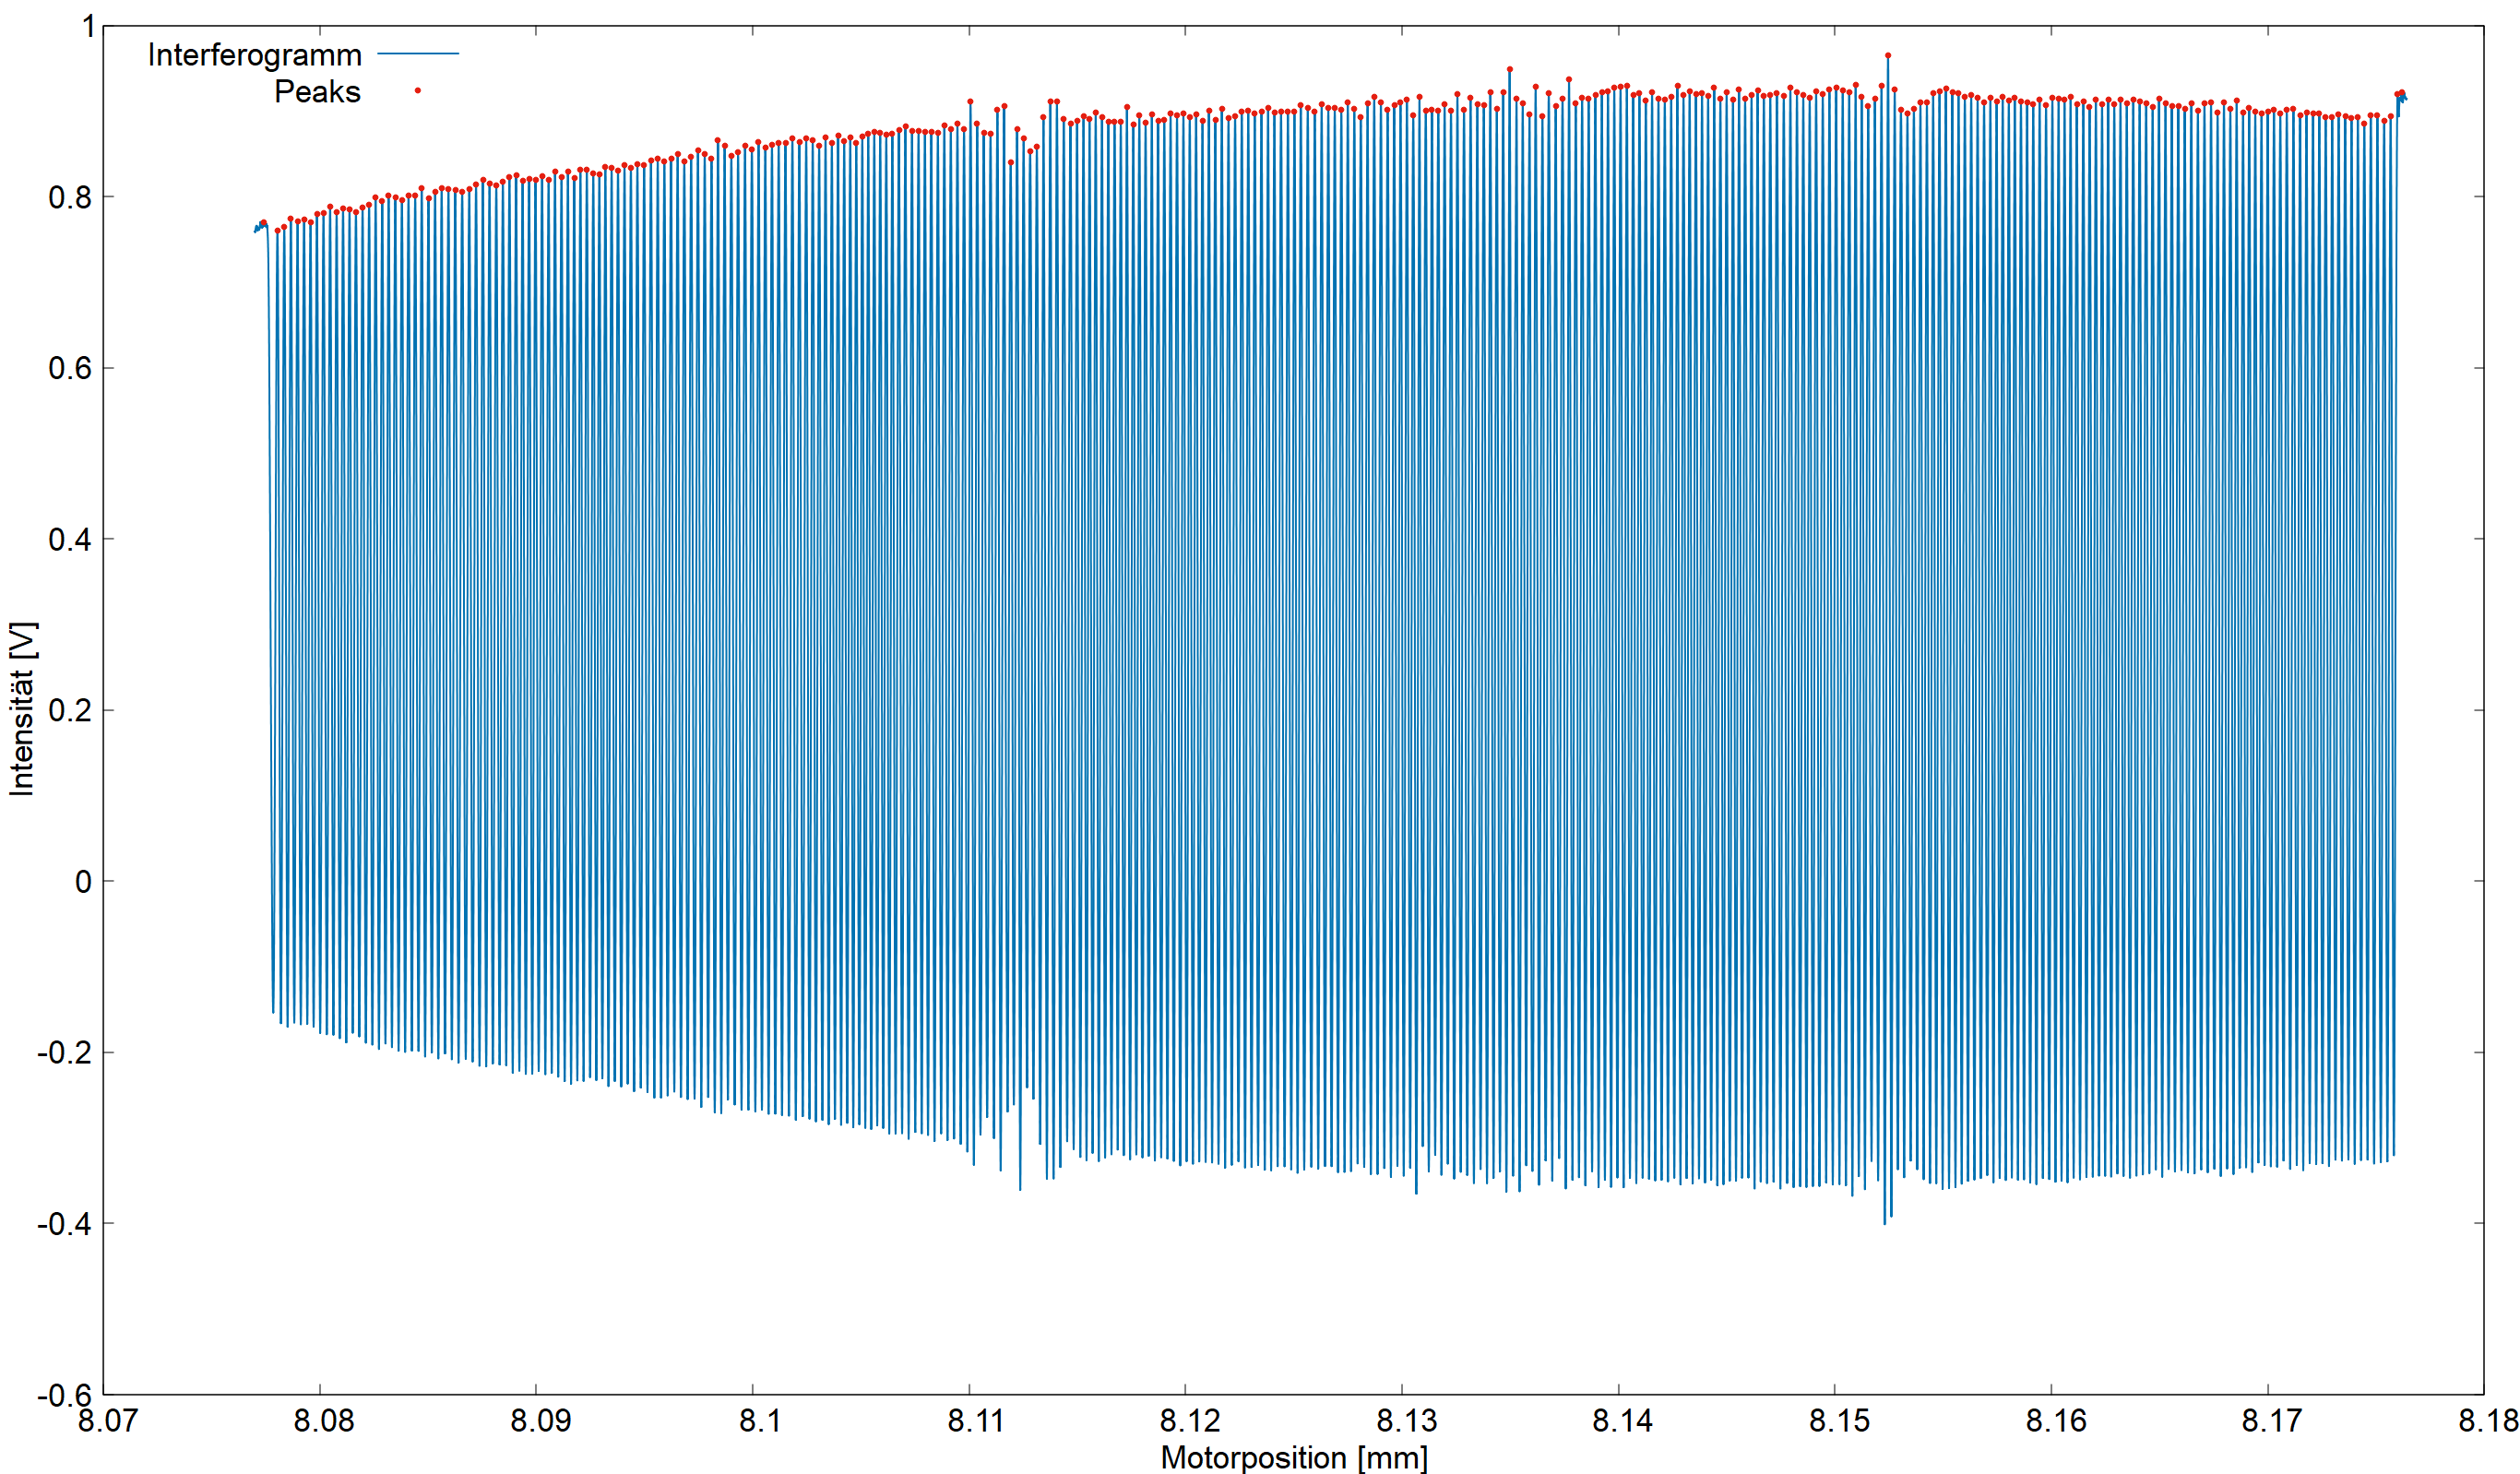
\includegraphics[width=\textwidth]{Dominik/test2.png}
    \caption{Interferogramm der Na-D Linie mit eingezeichneten Peaks.}
\end{figure}\\
Wenn man nun einen Ausschnitt etwas genauer betrachtet:
\begin{figure}[h]
    \centering\subfigure[Na-D Linie]{\scalebox{0.7}{% GNUPLOT: LaTeX picture with Postscript
\begingroup
  % Encoding inside the plot.  In the header of your document, this encoding
  % should to defined, e.g., by using
  % \usepackage[cp1252,<other encodings>]{inputenc}
  \inputencoding{cp1252}%
  \makeatletter
  \providecommand\color[2][]{%
    \GenericError{(gnuplot) \space\space\space\@spaces}{%
      Package color not loaded in conjunction with
      terminal option `colourtext'%
    }{See the gnuplot documentation for explanation.%
    }{Either use 'blacktext' in gnuplot or load the package
      color.sty in LaTeX.}%
    \renewcommand\color[2][]{}%
  }%
  \providecommand\includegraphics[2][]{%
    \GenericError{(gnuplot) \space\space\space\@spaces}{%
      Package graphicx or graphics not loaded%
    }{See the gnuplot documentation for explanation.%
    }{The gnuplot epslatex terminal needs graphicx.sty or graphics.sty.}%
    \renewcommand\includegraphics[2][]{}%
  }%
  \providecommand\rotatebox[2]{#2}%
  \@ifundefined{ifGPcolor}{%
    \newif\ifGPcolor
    \GPcolorfalse
  }{}%
  \@ifundefined{ifGPblacktext}{%
    \newif\ifGPblacktext
    \GPblacktexttrue
  }{}%
  % define a \g@addto@macro without @ in the name:
  \let\gplgaddtomacro\g@addto@macro
  % define empty templates for all commands taking text:
  \gdef\gplbacktext{}%
  \gdef\gplfronttext{}%
  \makeatother
  \ifGPblacktext
    % no textcolor at all
    \def\colorrgb#1{}%
    \def\colorgray#1{}%
  \else
    % gray or color?
    \ifGPcolor
      \def\colorrgb#1{\color[rgb]{#1}}%
      \def\colorgray#1{\color[gray]{#1}}%
      \expandafter\def\csname LTw\endcsname{\color{white}}%
      \expandafter\def\csname LTb\endcsname{\color{black}}%
      \expandafter\def\csname LTa\endcsname{\color{black}}%
      \expandafter\def\csname LT0\endcsname{\color[rgb]{1,0,0}}%
      \expandafter\def\csname LT1\endcsname{\color[rgb]{0,1,0}}%
      \expandafter\def\csname LT2\endcsname{\color[rgb]{0,0,1}}%
      \expandafter\def\csname LT3\endcsname{\color[rgb]{1,0,1}}%
      \expandafter\def\csname LT4\endcsname{\color[rgb]{0,1,1}}%
      \expandafter\def\csname LT5\endcsname{\color[rgb]{1,1,0}}%
      \expandafter\def\csname LT6\endcsname{\color[rgb]{0,0,0}}%
      \expandafter\def\csname LT7\endcsname{\color[rgb]{1,0.3,0}}%
      \expandafter\def\csname LT8\endcsname{\color[rgb]{0.5,0.5,0.5}}%
    \else
      % gray
      \def\colorrgb#1{\color{black}}%
      \def\colorgray#1{\color[gray]{#1}}%
      \expandafter\def\csname LTw\endcsname{\color{white}}%
      \expandafter\def\csname LTb\endcsname{\color{black}}%
      \expandafter\def\csname LTa\endcsname{\color{black}}%
      \expandafter\def\csname LT0\endcsname{\color{black}}%
      \expandafter\def\csname LT1\endcsname{\color{black}}%
      \expandafter\def\csname LT2\endcsname{\color{black}}%
      \expandafter\def\csname LT3\endcsname{\color{black}}%
      \expandafter\def\csname LT4\endcsname{\color{black}}%
      \expandafter\def\csname LT5\endcsname{\color{black}}%
      \expandafter\def\csname LT6\endcsname{\color{black}}%
      \expandafter\def\csname LT7\endcsname{\color{black}}%
      \expandafter\def\csname LT8\endcsname{\color{black}}%
    \fi
  \fi
    \setlength{\unitlength}{0.0500bp}%
    \ifx\gptboxheight\undefined%
      \newlength{\gptboxheight}%
      \newlength{\gptboxwidth}%
      \newsavebox{\gptboxtext}%
    \fi%
    \setlength{\fboxrule}{0.5pt}%
    \setlength{\fboxsep}{1pt}%
\begin{picture}(7200.00,5040.00)%
    \gplgaddtomacro\gplbacktext{%
      \csname LTb\endcsname%%
      \put(946,704){\makebox(0,0)[r]{\strut{}$-0.4$}}%
      \put(946,1253){\makebox(0,0)[r]{\strut{}$-0.2$}}%
      \put(946,1801){\makebox(0,0)[r]{\strut{}$0$}}%
      \put(946,2350){\makebox(0,0)[r]{\strut{}$0.2$}}%
      \put(946,2899){\makebox(0,0)[r]{\strut{}$0.4$}}%
      \put(946,3447){\makebox(0,0)[r]{\strut{}$0.6$}}%
      \put(946,3996){\makebox(0,0)[r]{\strut{}$0.8$}}%
      \put(946,4545){\makebox(0,0)[r]{\strut{}$1$}}%
      \put(1078,484){\makebox(0,0){\strut{}$8.12$}}%
      \put(2201,484){\makebox(0,0){\strut{}$8.122$}}%
      \put(3324,484){\makebox(0,0){\strut{}$8.124$}}%
      \put(4447,484){\makebox(0,0){\strut{}$8.126$}}%
      \put(5570,484){\makebox(0,0){\strut{}$8.128$}}%
      \put(6693,484){\makebox(0,0){\strut{}$8.13$}}%
    }%
    \gplgaddtomacro\gplfronttext{%
      \csname LTb\endcsname%%
      \put(209,2761){\rotatebox{-270}{\makebox(0,0){\strut{}Intensit\"at [V]}}}%
      \csname LTb\endcsname%%
      \put(6748,2761){\rotatebox{-270}{\makebox(0,0){\strut{}}}}%
      \csname LTb\endcsname%%
      \put(3885,154){\makebox(0,0){\strut{}Motorposition [mm]}}%
      \csname LTb\endcsname%%
      \put(3885,4819){\makebox(0,0){\strut{}}}%
      \csname LTb\endcsname%%
      \put(132,-110){\makebox(0,0)[l]{\strut{}}}%
      \csname LTb\endcsname%%
      \put(5706,4646){\makebox(0,0)[r]{\strut{}Interferogramm}}%
      \csname LTb\endcsname%%
      \put(5706,4426){\makebox(0,0)[r]{\strut{}Peaks}}%
    }%
    \gplbacktext
    \put(0,0){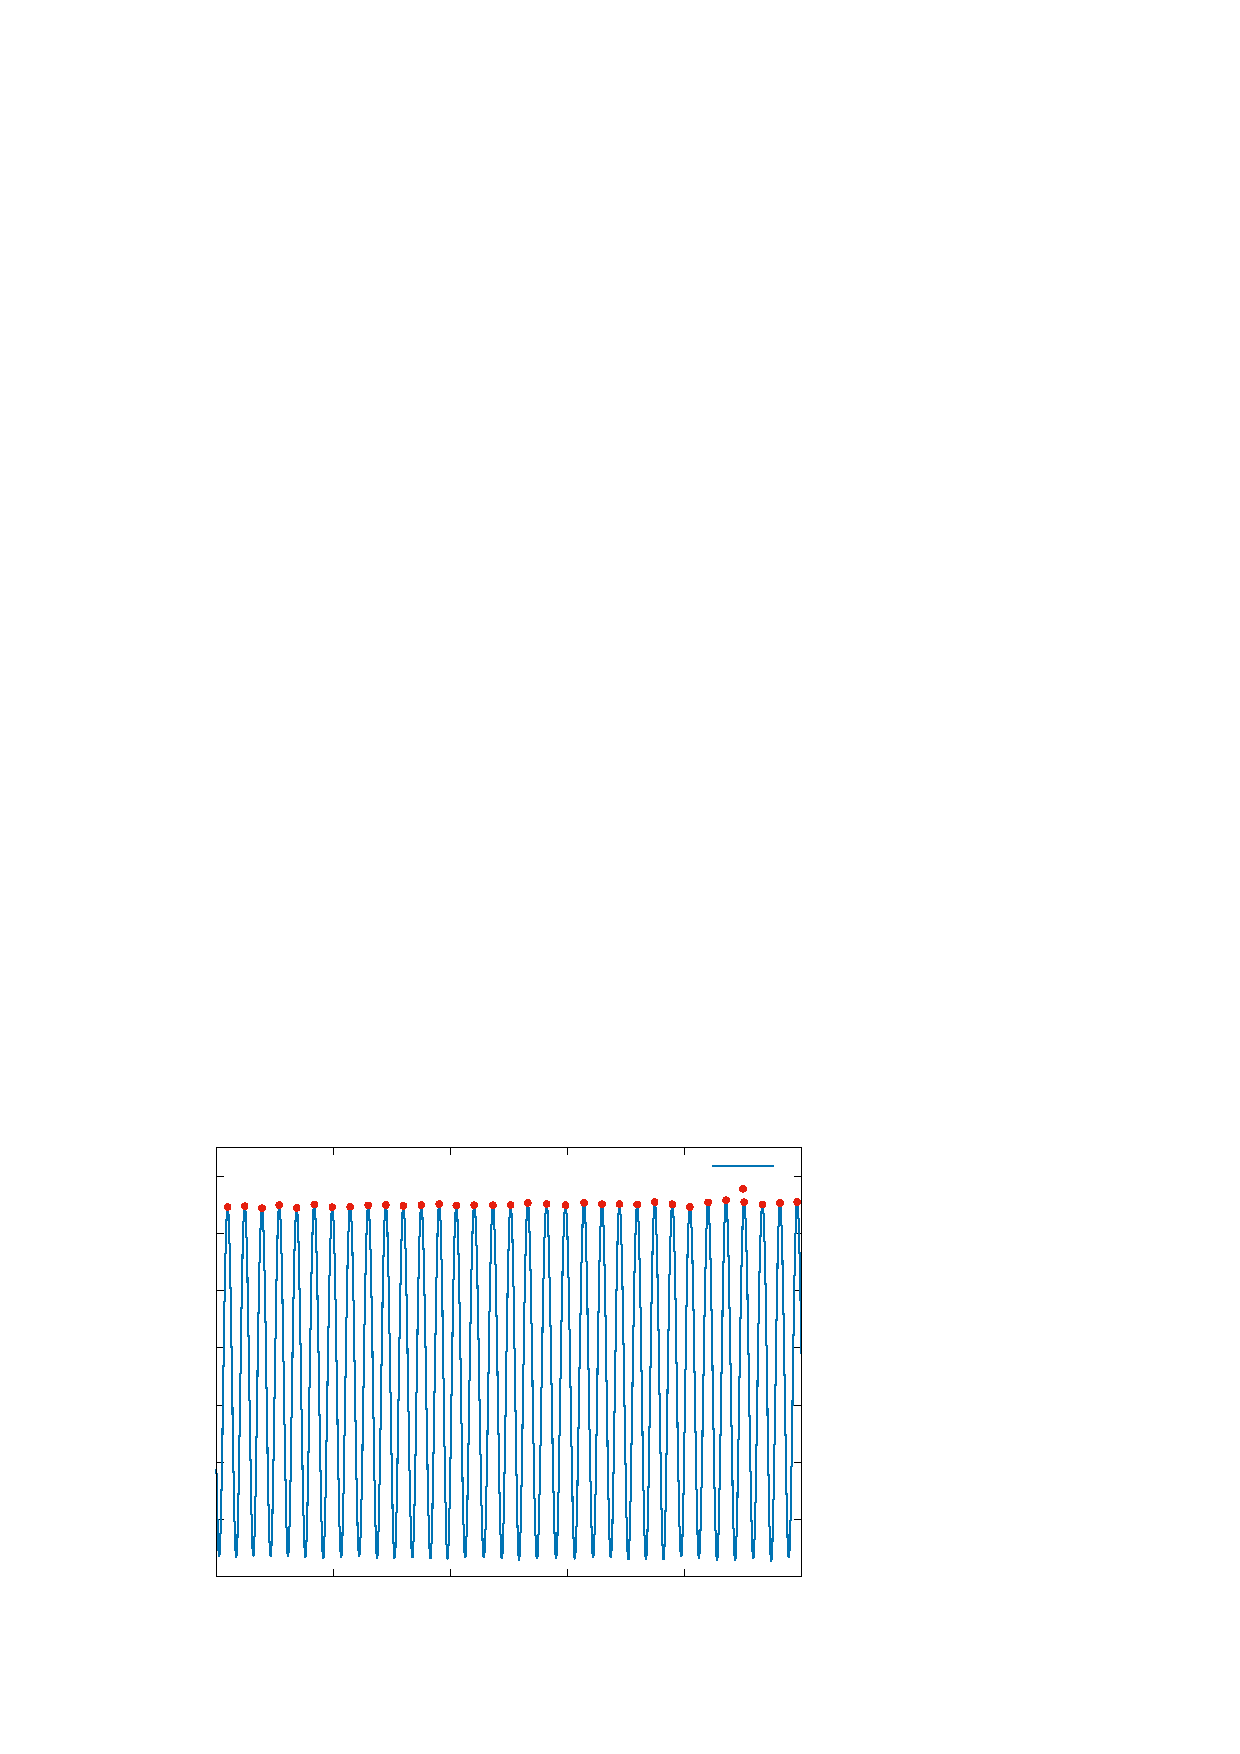
\includegraphics[width={360.00bp},height={252.00bp}]{Dominik/interferogram_na}}%
    \gplfronttext
  \end{picture}%
\endgroup
}}\\
    \subfigure[HeNe-Laser]{\scalebox{0.7}{% GNUPLOT: LaTeX picture with Postscript
\begingroup
  % Encoding inside the plot.  In the header of your document, this encoding
  % should to defined, e.g., by using
  % \usepackage[cp1252,<other encodings>]{inputenc}
  \inputencoding{cp1252}%
  \makeatletter
  \providecommand\color[2][]{%
    \GenericError{(gnuplot) \space\space\space\@spaces}{%
      Package color not loaded in conjunction with
      terminal option `colourtext'%
    }{See the gnuplot documentation for explanation.%
    }{Either use 'blacktext' in gnuplot or load the package
      color.sty in LaTeX.}%
    \renewcommand\color[2][]{}%
  }%
  \providecommand\includegraphics[2][]{%
    \GenericError{(gnuplot) \space\space\space\@spaces}{%
      Package graphicx or graphics not loaded%
    }{See the gnuplot documentation for explanation.%
    }{The gnuplot epslatex terminal needs graphicx.sty or graphics.sty.}%
    \renewcommand\includegraphics[2][]{}%
  }%
  \providecommand\rotatebox[2]{#2}%
  \@ifundefined{ifGPcolor}{%
    \newif\ifGPcolor
    \GPcolorfalse
  }{}%
  \@ifundefined{ifGPblacktext}{%
    \newif\ifGPblacktext
    \GPblacktexttrue
  }{}%
  % define a \g@addto@macro without @ in the name:
  \let\gplgaddtomacro\g@addto@macro
  % define empty templates for all commands taking text:
  \gdef\gplbacktext{}%
  \gdef\gplfronttext{}%
  \makeatother
  \ifGPblacktext
    % no textcolor at all
    \def\colorrgb#1{}%
    \def\colorgray#1{}%
  \else
    % gray or color?
    \ifGPcolor
      \def\colorrgb#1{\color[rgb]{#1}}%
      \def\colorgray#1{\color[gray]{#1}}%
      \expandafter\def\csname LTw\endcsname{\color{white}}%
      \expandafter\def\csname LTb\endcsname{\color{black}}%
      \expandafter\def\csname LTa\endcsname{\color{black}}%
      \expandafter\def\csname LT0\endcsname{\color[rgb]{1,0,0}}%
      \expandafter\def\csname LT1\endcsname{\color[rgb]{0,1,0}}%
      \expandafter\def\csname LT2\endcsname{\color[rgb]{0,0,1}}%
      \expandafter\def\csname LT3\endcsname{\color[rgb]{1,0,1}}%
      \expandafter\def\csname LT4\endcsname{\color[rgb]{0,1,1}}%
      \expandafter\def\csname LT5\endcsname{\color[rgb]{1,1,0}}%
      \expandafter\def\csname LT6\endcsname{\color[rgb]{0,0,0}}%
      \expandafter\def\csname LT7\endcsname{\color[rgb]{1,0.3,0}}%
      \expandafter\def\csname LT8\endcsname{\color[rgb]{0.5,0.5,0.5}}%
    \else
      % gray
      \def\colorrgb#1{\color{black}}%
      \def\colorgray#1{\color[gray]{#1}}%
      \expandafter\def\csname LTw\endcsname{\color{white}}%
      \expandafter\def\csname LTb\endcsname{\color{black}}%
      \expandafter\def\csname LTa\endcsname{\color{black}}%
      \expandafter\def\csname LT0\endcsname{\color{black}}%
      \expandafter\def\csname LT1\endcsname{\color{black}}%
      \expandafter\def\csname LT2\endcsname{\color{black}}%
      \expandafter\def\csname LT3\endcsname{\color{black}}%
      \expandafter\def\csname LT4\endcsname{\color{black}}%
      \expandafter\def\csname LT5\endcsname{\color{black}}%
      \expandafter\def\csname LT6\endcsname{\color{black}}%
      \expandafter\def\csname LT7\endcsname{\color{black}}%
      \expandafter\def\csname LT8\endcsname{\color{black}}%
    \fi
  \fi
    \setlength{\unitlength}{0.0500bp}%
    \ifx\gptboxheight\undefined%
      \newlength{\gptboxheight}%
      \newlength{\gptboxwidth}%
      \newsavebox{\gptboxtext}%
    \fi%
    \setlength{\fboxrule}{0.5pt}%
    \setlength{\fboxsep}{1pt}%
\begin{picture}(7200.00,5040.00)%
    \gplgaddtomacro\gplbacktext{%
      \csname LTb\endcsname%%
      \put(946,704){\makebox(0,0)[r]{\strut{}$-0.1$}}%
      \put(946,1218){\makebox(0,0)[r]{\strut{}$0$}}%
      \put(946,1733){\makebox(0,0)[r]{\strut{}$0.1$}}%
      \put(946,2247){\makebox(0,0)[r]{\strut{}$0.2$}}%
      \put(946,2762){\makebox(0,0)[r]{\strut{}$0.3$}}%
      \put(946,3276){\makebox(0,0)[r]{\strut{}$0.4$}}%
      \put(946,3790){\makebox(0,0)[r]{\strut{}$0.5$}}%
      \put(946,4305){\makebox(0,0)[r]{\strut{}$0.6$}}%
      \put(946,4819){\makebox(0,0)[r]{\strut{}$0.7$}}%
      \put(1078,484){\makebox(0,0){\strut{}$8.12$}}%
      \put(2223,484){\makebox(0,0){\strut{}$8.122$}}%
      \put(3368,484){\makebox(0,0){\strut{}$8.124$}}%
      \put(4513,484){\makebox(0,0){\strut{}$8.126$}}%
      \put(5658,484){\makebox(0,0){\strut{}$8.128$}}%
      \put(6803,484){\makebox(0,0){\strut{}$8.13$}}%
    }%
    \gplgaddtomacro\gplfronttext{%
      \csname LTb\endcsname%%
      \put(209,2761){\rotatebox{-270}{\makebox(0,0){\strut{}Intensit\"at [V]}}}%
      \put(3940,154){\makebox(0,0){\strut{}Motorposition [mm]}}%
      \csname LTb\endcsname%%
      \put(5816,4646){\makebox(0,0)[r]{\strut{}Interferogramm}}%
      \csname LTb\endcsname%%
      \put(5816,4426){\makebox(0,0)[r]{\strut{}Peaks}}%
    }%
    \gplbacktext
    \put(0,0){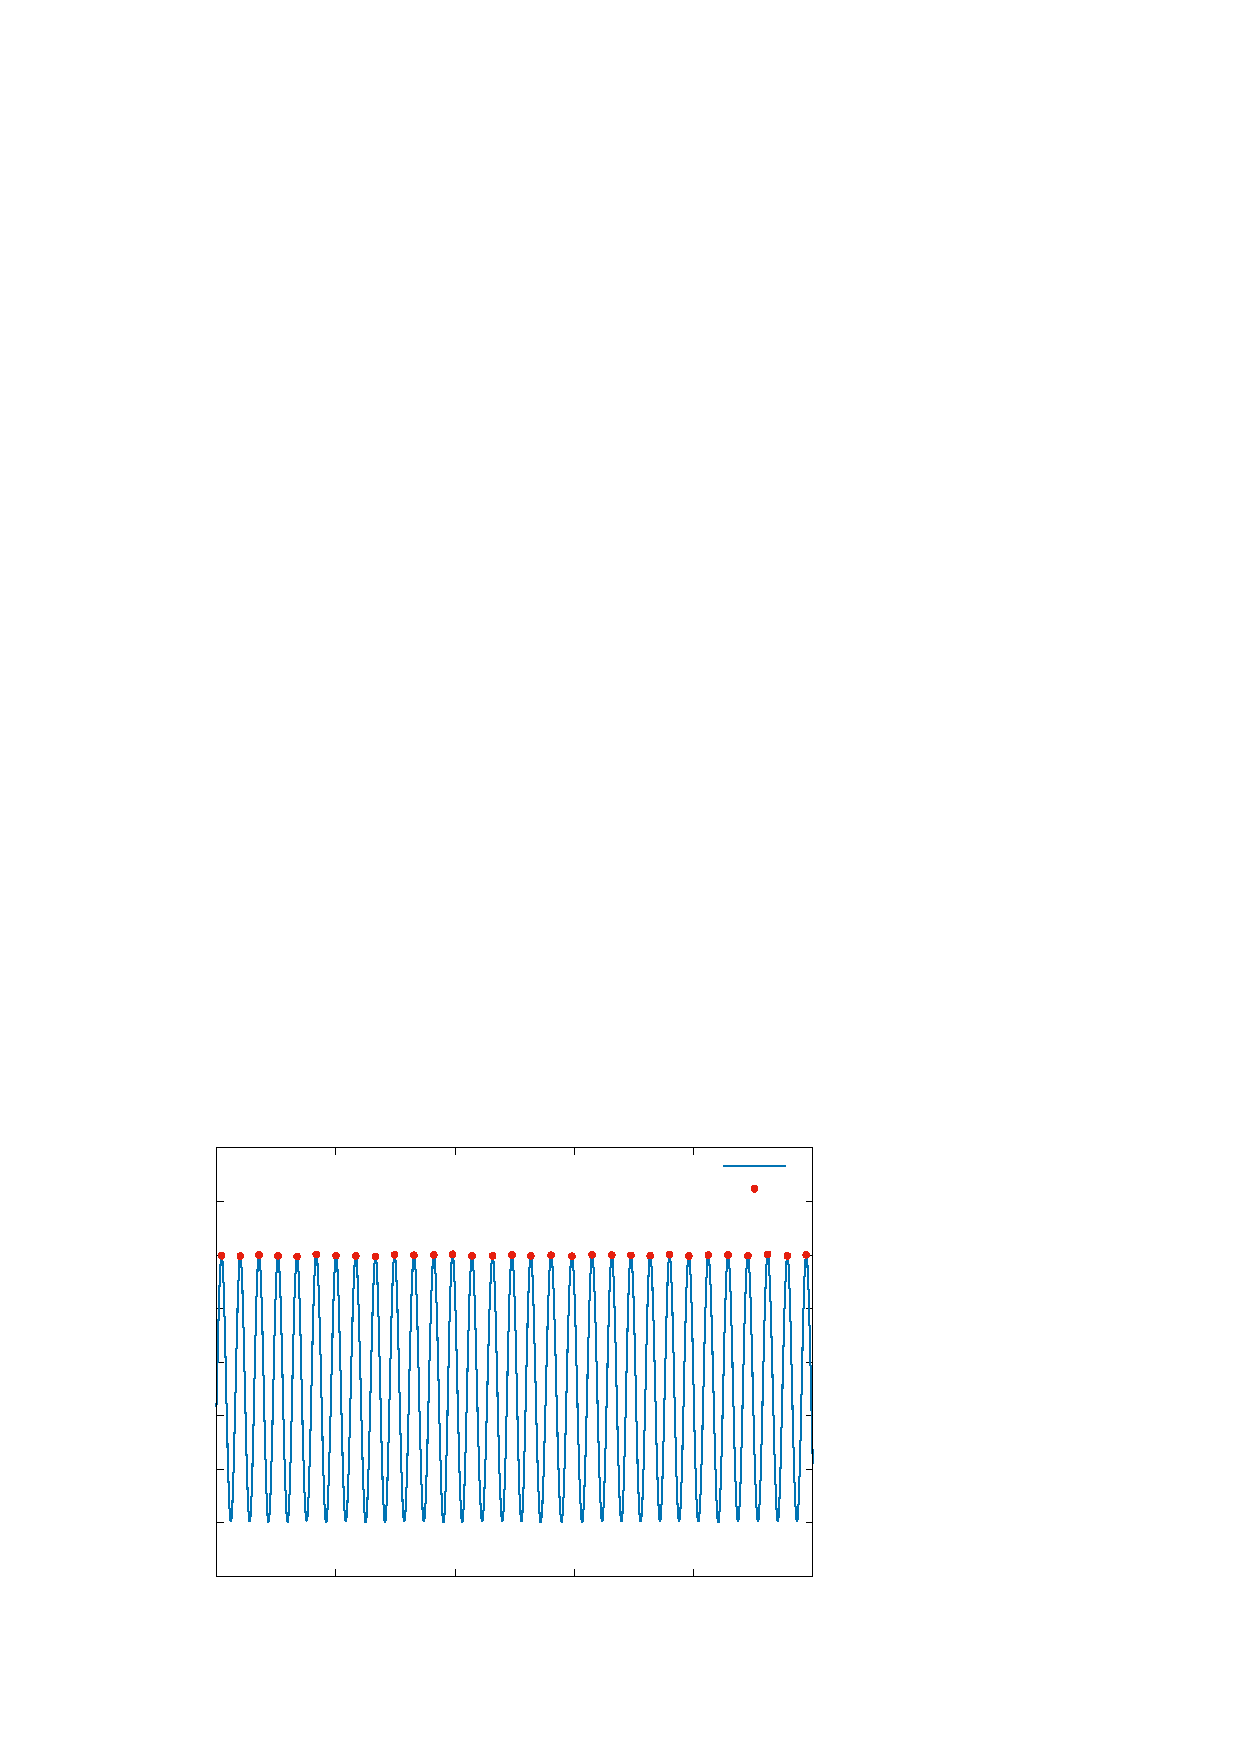
\includegraphics[width={360.00bp},height={252.00bp}]{Dominik/interferogram_nala}}%
    \gplfronttext
  \end{picture}%
\endgroup
}}
    \caption{Ausschnitt aus dem Interferogrammen der Na-D Linie (a) und des HeNe-Lasers (b) mit eingezeichneten Peaks}
\end{figure}\newpage
Wir nehmen an, dass der Peak-finder die Peaks bis zu einen Peak genau findet.
Somit folgt für die Peaks im Spektrum der Natriumdampflampe:
\begin{equation}
    n_{Na}=331\pm1
\end{equation}
Und für den Lasers:
\begin{equation}
    n_{Laser}=307\pm1
\end{equation}
Somit folgt für die Wellenlänge der Natriumdampflampe:
\begin{equation}
    \lambda_{Na}=\left(587\pm3\right)\,\text{nm}
\end{equation}
Der Fehler wurde über eine Fehlerfortpflanzung berechnet:
\begin{align}
    s_{\lambda} &= \sqrt{\left(\frac{\partial \lambda_{Na}}{\partial n_{Laser}}\cdot s_{n_{Laser}}\right)^2+ \left(\frac{\partial \lambda_{Na}}{\partial n_{Na}}\cdot s_{n_{Na}}\right)^2}\\
                &= \sqrt{\left(\frac{\lambda_L}{n_{Na}} \cdot s_{n_{Laser}}\right)^2 + \left(\frac{\lambda_L \cdot n_L}{n^2_{Na}} \cdot s_{n_{Na}}\right)^2 }
\end{align}
Wenn man nun den gemessenen Wert der Natrium-D Linie mit den theoretischen Werten der Natrium-D Linie vergleicht $(\lambda_{D1}=589,593\,\text{nm}; \lambda_{D2}=588,996\,\text{nm})$, sieht man das der gemessene Wert mit seinen Fehler die tatsächlichen Werte einschließt.
%Die so bestimmte Wellenlänge mit ihrem Fehler schließen die theoretischen Werte der Natrium-D Linien ein.

\subsubsection{Kohärenzlänge bestimmen}
Die Kohärenzlänge ist die halbe Intervalllänge der Einhüllenden, bei dieser die maximale Intensität  auf $1/e$ abgefallen ist.
Diese kann man direkt aus der Einhüllenden herauslesen.
Für die maximale Intensität wurde gemessen:
\begin{align}
    I_0&=\left(0,0883\pm0,0001\right)\,\text{V}\\ %y-Achsenabstand: 0,0278
    \frac{I_0}{e}&=\left(32,48\pm0,04\right)\,\text{mV}
\end{align}
Hierbei wurde der y-Achsen Offset der Messkurve berücksichtigt.
Dieser ist die Differenz zwischen dem Nullwert des Plots und des Wertes auf den die Intensität abfällt.
%Der y-Achsen Offset ist der Wert, auf den die Linie abfällt, anstatt das diese auf Null abfällt.\\
Somit folgt für die Kohärenzlänge $L$:
\begin{align}
    L&=\beta\cdot\frac{\Delta s\left(\frac{I_0}{e}\right)}{2}\\
    L&=\left(2,5\pm0,1\right)\,\text{mm}
\end{align}\newpage
Graphisch folgt:
\begin{figure}[h]
    \centering\scalebox{0.8}{% GNUPLOT: LaTeX picture with Postscript
\begingroup
  % Encoding inside the plot.  In the header of your document, this encoding
  % should to defined, e.g., by using
  % \usepackage[cp1252,<other encodings>]{inputenc}
  \inputencoding{cp1252}%
  \makeatletter
  \providecommand\color[2][]{%
    \GenericError{(gnuplot) \space\space\space\@spaces}{%
      Package color not loaded in conjunction with
      terminal option `colourtext'%
    }{See the gnuplot documentation for explanation.%
    }{Either use 'blacktext' in gnuplot or load the package
      color.sty in LaTeX.}%
    \renewcommand\color[2][]{}%
  }%
  \providecommand\includegraphics[2][]{%
    \GenericError{(gnuplot) \space\space\space\@spaces}{%
      Package graphicx or graphics not loaded%
    }{See the gnuplot documentation for explanation.%
    }{The gnuplot epslatex terminal needs graphicx.sty or graphics.sty.}%
    \renewcommand\includegraphics[2][]{}%
  }%
  \providecommand\rotatebox[2]{#2}%
  \@ifundefined{ifGPcolor}{%
    \newif\ifGPcolor
    \GPcolorfalse
  }{}%
  \@ifundefined{ifGPblacktext}{%
    \newif\ifGPblacktext
    \GPblacktexttrue
  }{}%
  % define a \g@addto@macro without @ in the name:
  \let\gplgaddtomacro\g@addto@macro
  % define empty templates for all commands taking text:
  \gdef\gplbacktext{}%
  \gdef\gplfronttext{}%
  \makeatother
  \ifGPblacktext
    % no textcolor at all
    \def\colorrgb#1{}%
    \def\colorgray#1{}%
  \else
    % gray or color?
    \ifGPcolor
      \def\colorrgb#1{\color[rgb]{#1}}%
      \def\colorgray#1{\color[gray]{#1}}%
      \expandafter\def\csname LTw\endcsname{\color{white}}%
      \expandafter\def\csname LTb\endcsname{\color{black}}%
      \expandafter\def\csname LTa\endcsname{\color{black}}%
      \expandafter\def\csname LT0\endcsname{\color[rgb]{1,0,0}}%
      \expandafter\def\csname LT1\endcsname{\color[rgb]{0,1,0}}%
      \expandafter\def\csname LT2\endcsname{\color[rgb]{0,0,1}}%
      \expandafter\def\csname LT3\endcsname{\color[rgb]{1,0,1}}%
      \expandafter\def\csname LT4\endcsname{\color[rgb]{0,1,1}}%
      \expandafter\def\csname LT5\endcsname{\color[rgb]{1,1,0}}%
      \expandafter\def\csname LT6\endcsname{\color[rgb]{0,0,0}}%
      \expandafter\def\csname LT7\endcsname{\color[rgb]{1,0.3,0}}%
      \expandafter\def\csname LT8\endcsname{\color[rgb]{0.5,0.5,0.5}}%
    \else
      % gray
      \def\colorrgb#1{\color{black}}%
      \def\colorgray#1{\color[gray]{#1}}%
      \expandafter\def\csname LTw\endcsname{\color{white}}%
      \expandafter\def\csname LTb\endcsname{\color{black}}%
      \expandafter\def\csname LTa\endcsname{\color{black}}%
      \expandafter\def\csname LT0\endcsname{\color{black}}%
      \expandafter\def\csname LT1\endcsname{\color{black}}%
      \expandafter\def\csname LT2\endcsname{\color{black}}%
      \expandafter\def\csname LT3\endcsname{\color{black}}%
      \expandafter\def\csname LT4\endcsname{\color{black}}%
      \expandafter\def\csname LT5\endcsname{\color{black}}%
      \expandafter\def\csname LT6\endcsname{\color{black}}%
      \expandafter\def\csname LT7\endcsname{\color{black}}%
      \expandafter\def\csname LT8\endcsname{\color{black}}%
    \fi
  \fi
    \setlength{\unitlength}{0.0500bp}%
    \ifx\gptboxheight\undefined%
      \newlength{\gptboxheight}%
      \newlength{\gptboxwidth}%
      \newsavebox{\gptboxtext}%
    \fi%
    \setlength{\fboxrule}{0.5pt}%
    \setlength{\fboxsep}{1pt}%
\begin{picture}(7200.00,5040.00)%
    \gplgaddtomacro\gplbacktext{%
      \csname LTb\endcsname%%
      \put(946,704){\makebox(0,0)[r]{\strut{}$0.02$}}%
      \put(946,1116){\makebox(0,0)[r]{\strut{}$0.03$}}%
      \put(946,1527){\makebox(0,0)[r]{\strut{}$0.04$}}%
      \put(946,1939){\makebox(0,0)[r]{\strut{}$0.05$}}%
      \put(946,2350){\makebox(0,0)[r]{\strut{}$0.06$}}%
      \put(946,2761){\makebox(0,0)[r]{\strut{}$0.07$}}%
      \put(946,3173){\makebox(0,0)[r]{\strut{}$0.08$}}%
      \put(946,3585){\makebox(0,0)[r]{\strut{}$0.09$}}%
      \put(946,3996){\makebox(0,0)[r]{\strut{}$0.1$}}%
      \put(946,4408){\makebox(0,0)[r]{\strut{}$0.11$}}%
      \put(946,4819){\makebox(0,0)[r]{\strut{}$0.12$}}%
      \put(1078,484){\makebox(0,0){\strut{}$30$}}%
      \put(1598,484){\makebox(0,0){\strut{}$32$}}%
      \put(2119,484){\makebox(0,0){\strut{}$34$}}%
      \put(2639,484){\makebox(0,0){\strut{}$36$}}%
      \put(3160,484){\makebox(0,0){\strut{}$38$}}%
      \put(3680,484){\makebox(0,0){\strut{}$40$}}%
      \put(4201,484){\makebox(0,0){\strut{}$42$}}%
      \put(4721,484){\makebox(0,0){\strut{}$44$}}%
      \put(5242,484){\makebox(0,0){\strut{}$46$}}%
      \put(5762,484){\makebox(0,0){\strut{}$48$}}%
      \put(6283,484){\makebox(0,0){\strut{}$50$}}%
      \put(6803,484){\makebox(0,0){\strut{}$52$}}%
    }%
    \gplgaddtomacro\gplfronttext{%
      \csname LTb\endcsname%%
      \put(209,2761){\rotatebox{-270}{\makebox(0,0){\strut{}Intensit\"at [V]}}}%
      \put(3940,154){\makebox(0,0){\strut{}Motorposition [mm]}}%
    }%
    \gplbacktext
    \put(0,0){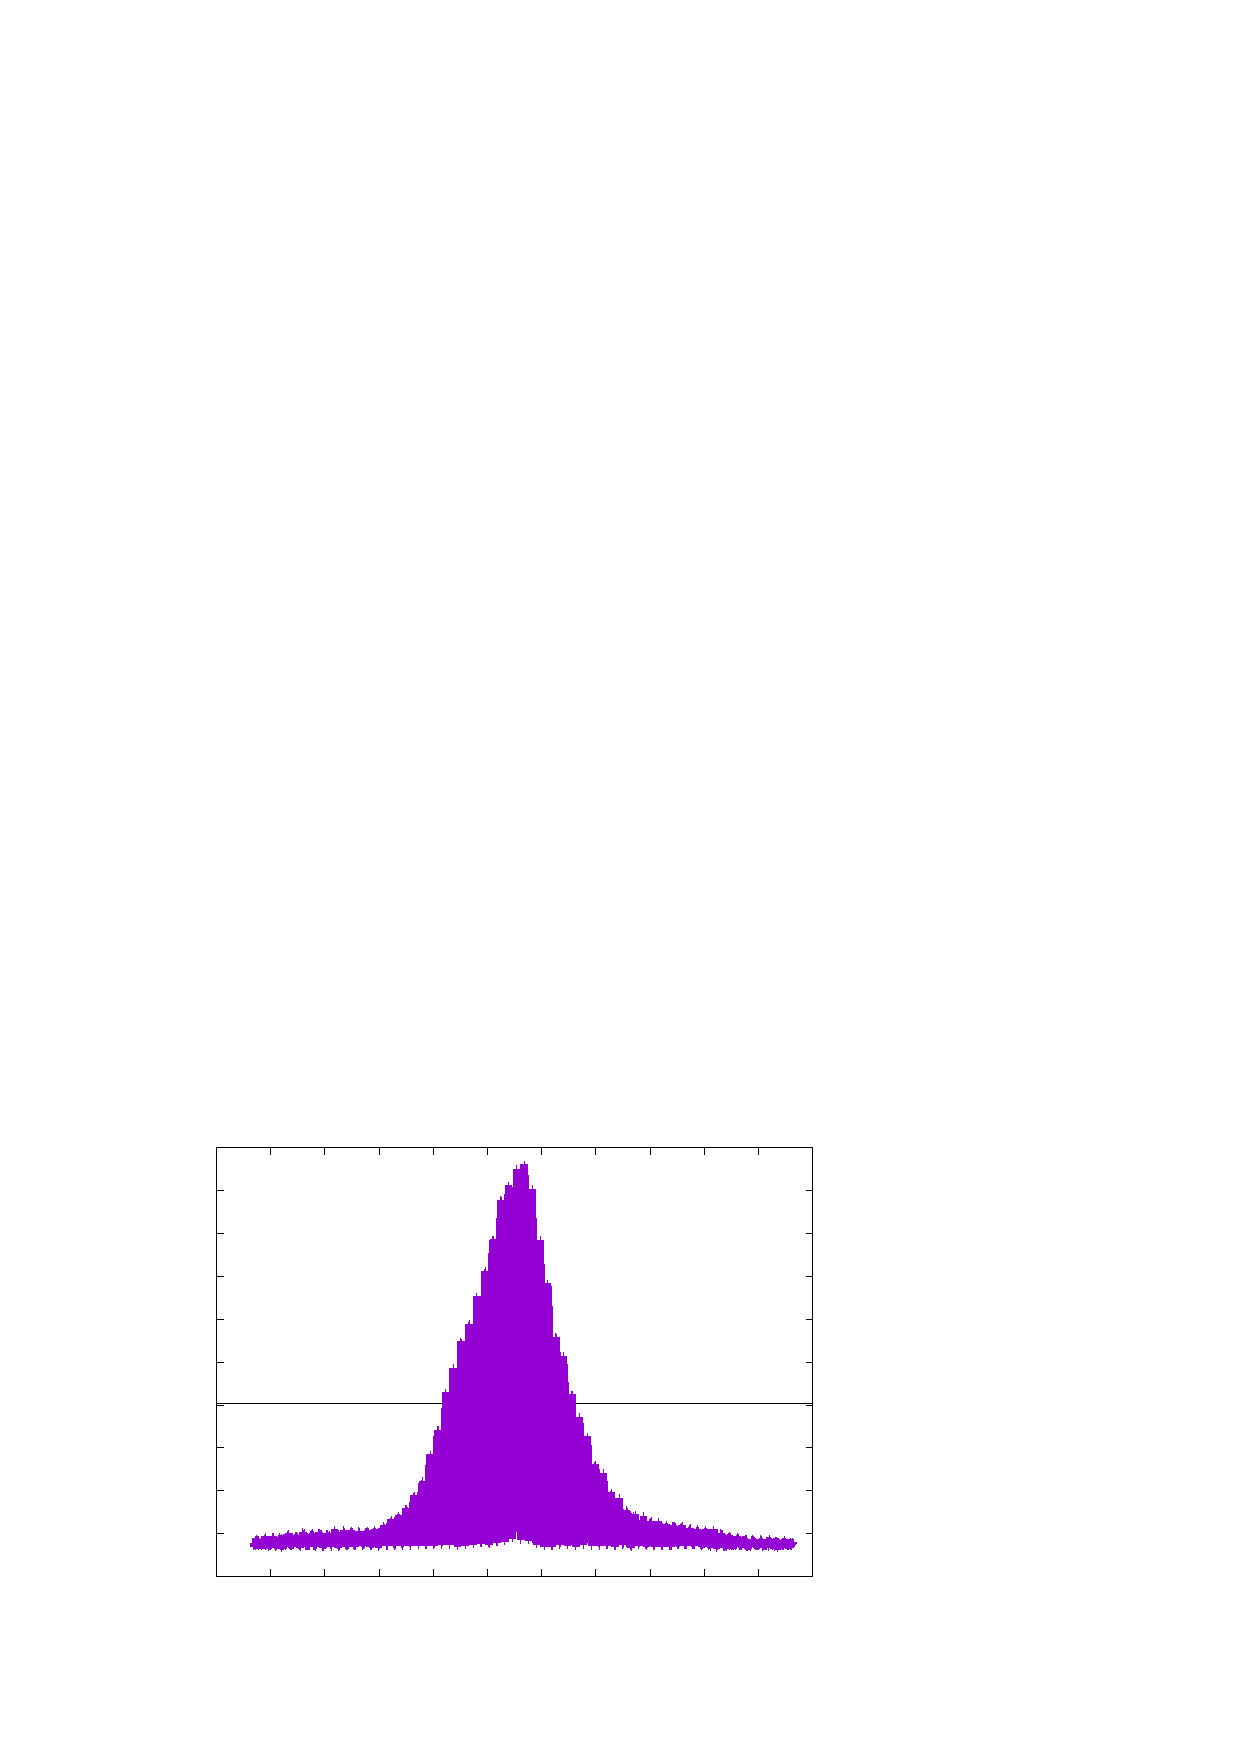
\includegraphics[width={360.00bp},height={252.00bp}]{Dominik/einhuellende_na_I}}%
    \gplfronttext
  \end{picture}%
\endgroup
}
    \caption{Einhüllende des Interferogramms der Na-D Linie mit eingezeichneter $I_0/e$-Intensität}
\end{figure}\\
Da die Einhüllende für die Schnittpunkte mit der $I_0/e$-Gerade per Augenmaß abgelesen wurde, nehmen wir einen Ablesefehler von $0,1\,\text{mm}$ an.
\subsubsection{Linienbreite bestimmen}
Um die Linienbreite zu berechnen muss man erst wissen, um welchen Verbreiterungsmechanismus es sich handelt.
Da die Kurve einer Gauß-Glocke ähnelt, liegt hier eine Dopplerverbreiterung vor (siehe \ref{abbildung_ein}).
Ein Fit dazu findet sich im Kapitel 'Verbreiterungsmechanismus' wieder.
Für diese wurden in den Fragen zur Vorbereitung die Umrechnung zwischen Linienbreite (FWHM-Breite) und Kohärenzlänge (halbe $1/e$-Breite) bestimmt.
Es ist hierbei zu beachten, dass die Linienbreite im k-Raum ausgerechnet wird (Wellenzahlen), um diese nun in den l-Raum umzurechnen folgt:
\begin{align}
    \left|\frac{\Delta k}{\Delta \lambda}\right|&=\left|\frac{dk}{d\lambda}\right|=\frac{2\pi}{\lambda^2}\\
    d\lambda&=dk\cdot\frac{\lambda^2}{2\pi}
\end{align}
Hier steht $dk$ für die FHWM-Breite der Linie im k-Raum, $\lambda$ für gemessene Wellenlänge und $d\lambda$ für die FWHM-Breite im l-Raum.\\
Somit folgt für die Linienbreite einer Dopplerverbreiterten Linie im l-Raum:
\begin{equation}
    \Delta \lambda_{Na}=\left(0,073\pm0,003\right)\,\text{nm}
\end{equation}
Der Fehler wurde über Fehlerfortpflanzung bestimmt:
\begin{align}
    s_{\Delta \lambda_{Na}} &= \sqrt{\left(\frac{\partial \Delta \lambda_{Na}}{\partial L_c} \cdot s_{L_c}\right)^2+\left(\frac{\partial \Delta \lambda_{Na}}{\partial \lambda_{Na}} \cdot s_{\lambda_{Na}}\right)^2} \\
    &= \sqrt{\left(\frac{2 \sqrt{ln(2)} \cdot \lambda^2_{Na}}{L_c^2 \cdot \pi} \cdot s_{L_c}\right)^2+\left(\frac{4 \sqrt{ln(2)}\cdot \lambda_{Na}}{L_c \cdot \pi} \cdot s_{\lambda_{Na}}\right)^2}
\end{align}
\newpage
\subsection{Intensitätsverhältnis und Abstand der beiden Natrium D-Linien}
Bei der Natriumdampflampe liegen die Linien, der D-1 und D-2 Linie sehr nahe zusammen, dies führt zu einer Schwebung.
\begin{figure}[h]
    \centering\scalebox{0.8}{% GNUPLOT: LaTeX picture with Postscript
\begingroup
  % Encoding inside the plot.  In the header of your document, this encoding
  % should to defined, e.g., by using
  % \usepackage[cp1252,<other encodings>]{inputenc}
  \inputencoding{cp1252}%
  \makeatletter
  \providecommand\color[2][]{%
    \GenericError{(gnuplot) \space\space\space\@spaces}{%
      Package color not loaded in conjunction with
      terminal option `colourtext'%
    }{See the gnuplot documentation for explanation.%
    }{Either use 'blacktext' in gnuplot or load the package
      color.sty in LaTeX.}%
    \renewcommand\color[2][]{}%
  }%
  \providecommand\includegraphics[2][]{%
    \GenericError{(gnuplot) \space\space\space\@spaces}{%
      Package graphicx or graphics not loaded%
    }{See the gnuplot documentation for explanation.%
    }{The gnuplot epslatex terminal needs graphicx.sty or graphics.sty.}%
    \renewcommand\includegraphics[2][]{}%
  }%
  \providecommand\rotatebox[2]{#2}%
  \@ifundefined{ifGPcolor}{%
    \newif\ifGPcolor
    \GPcolorfalse
  }{}%
  \@ifundefined{ifGPblacktext}{%
    \newif\ifGPblacktext
    \GPblacktexttrue
  }{}%
  % define a \g@addto@macro without @ in the name:
  \let\gplgaddtomacro\g@addto@macro
  % define empty templates for all commands taking text:
  \gdef\gplbacktext{}%
  \gdef\gplfronttext{}%
  \makeatother
  \ifGPblacktext
    % no textcolor at all
    \def\colorrgb#1{}%
    \def\colorgray#1{}%
  \else
    % gray or color?
    \ifGPcolor
      \def\colorrgb#1{\color[rgb]{#1}}%
      \def\colorgray#1{\color[gray]{#1}}%
      \expandafter\def\csname LTw\endcsname{\color{white}}%
      \expandafter\def\csname LTb\endcsname{\color{black}}%
      \expandafter\def\csname LTa\endcsname{\color{black}}%
      \expandafter\def\csname LT0\endcsname{\color[rgb]{1,0,0}}%
      \expandafter\def\csname LT1\endcsname{\color[rgb]{0,1,0}}%
      \expandafter\def\csname LT2\endcsname{\color[rgb]{0,0,1}}%
      \expandafter\def\csname LT3\endcsname{\color[rgb]{1,0,1}}%
      \expandafter\def\csname LT4\endcsname{\color[rgb]{0,1,1}}%
      \expandafter\def\csname LT5\endcsname{\color[rgb]{1,1,0}}%
      \expandafter\def\csname LT6\endcsname{\color[rgb]{0,0,0}}%
      \expandafter\def\csname LT7\endcsname{\color[rgb]{1,0.3,0}}%
      \expandafter\def\csname LT8\endcsname{\color[rgb]{0.5,0.5,0.5}}%
    \else
      % gray
      \def\colorrgb#1{\color{black}}%
      \def\colorgray#1{\color[gray]{#1}}%
      \expandafter\def\csname LTw\endcsname{\color{white}}%
      \expandafter\def\csname LTb\endcsname{\color{black}}%
      \expandafter\def\csname LTa\endcsname{\color{black}}%
      \expandafter\def\csname LT0\endcsname{\color{black}}%
      \expandafter\def\csname LT1\endcsname{\color{black}}%
      \expandafter\def\csname LT2\endcsname{\color{black}}%
      \expandafter\def\csname LT3\endcsname{\color{black}}%
      \expandafter\def\csname LT4\endcsname{\color{black}}%
      \expandafter\def\csname LT5\endcsname{\color{black}}%
      \expandafter\def\csname LT6\endcsname{\color{black}}%
      \expandafter\def\csname LT7\endcsname{\color{black}}%
      \expandafter\def\csname LT8\endcsname{\color{black}}%
    \fi
  \fi
    \setlength{\unitlength}{0.0500bp}%
    \ifx\gptboxheight\undefined%
      \newlength{\gptboxheight}%
      \newlength{\gptboxwidth}%
      \newsavebox{\gptboxtext}%
    \fi%
    \setlength{\fboxrule}{0.5pt}%
    \setlength{\fboxsep}{1pt}%
\begin{picture}(7200.00,5040.00)%
    \gplgaddtomacro\gplbacktext{%
      \csname LTb\endcsname%%
      \put(946,704){\makebox(0,0)[r]{\strut{}$-0.4$}}%
      \put(946,1292){\makebox(0,0)[r]{\strut{}$-0.2$}}%
      \put(946,1880){\makebox(0,0)[r]{\strut{}$0$}}%
      \put(946,2468){\makebox(0,0)[r]{\strut{}$0.2$}}%
      \put(946,3055){\makebox(0,0)[r]{\strut{}$0.4$}}%
      \put(946,3643){\makebox(0,0)[r]{\strut{}$0.6$}}%
      \put(946,4231){\makebox(0,0)[r]{\strut{}$0.8$}}%
      \put(946,4819){\makebox(0,0)[r]{\strut{}$1$}}%
      \put(1078,484){\makebox(0,0){\strut{}$7.95$}}%
      \put(1794,484){\makebox(0,0){\strut{}$8$}}%
      \put(2509,484){\makebox(0,0){\strut{}$8.05$}}%
      \put(3225,484){\makebox(0,0){\strut{}$8.1$}}%
      \put(3941,484){\makebox(0,0){\strut{}$8.15$}}%
      \put(4656,484){\makebox(0,0){\strut{}$8.2$}}%
      \put(5372,484){\makebox(0,0){\strut{}$8.25$}}%
      \put(6087,484){\makebox(0,0){\strut{}$8.3$}}%
      \put(6803,484){\makebox(0,0){\strut{}$8.35$}}%
    }%
    \gplgaddtomacro\gplfronttext{%
      \csname LTb\endcsname%%
      \put(209,2761){\rotatebox{-270}{\makebox(0,0){\strut{}Intensit\"at [V]}}}%
      \put(3940,154){\makebox(0,0){\strut{}Motorposition [mm]}}%
    }%
    \gplbacktext
    \put(0,0){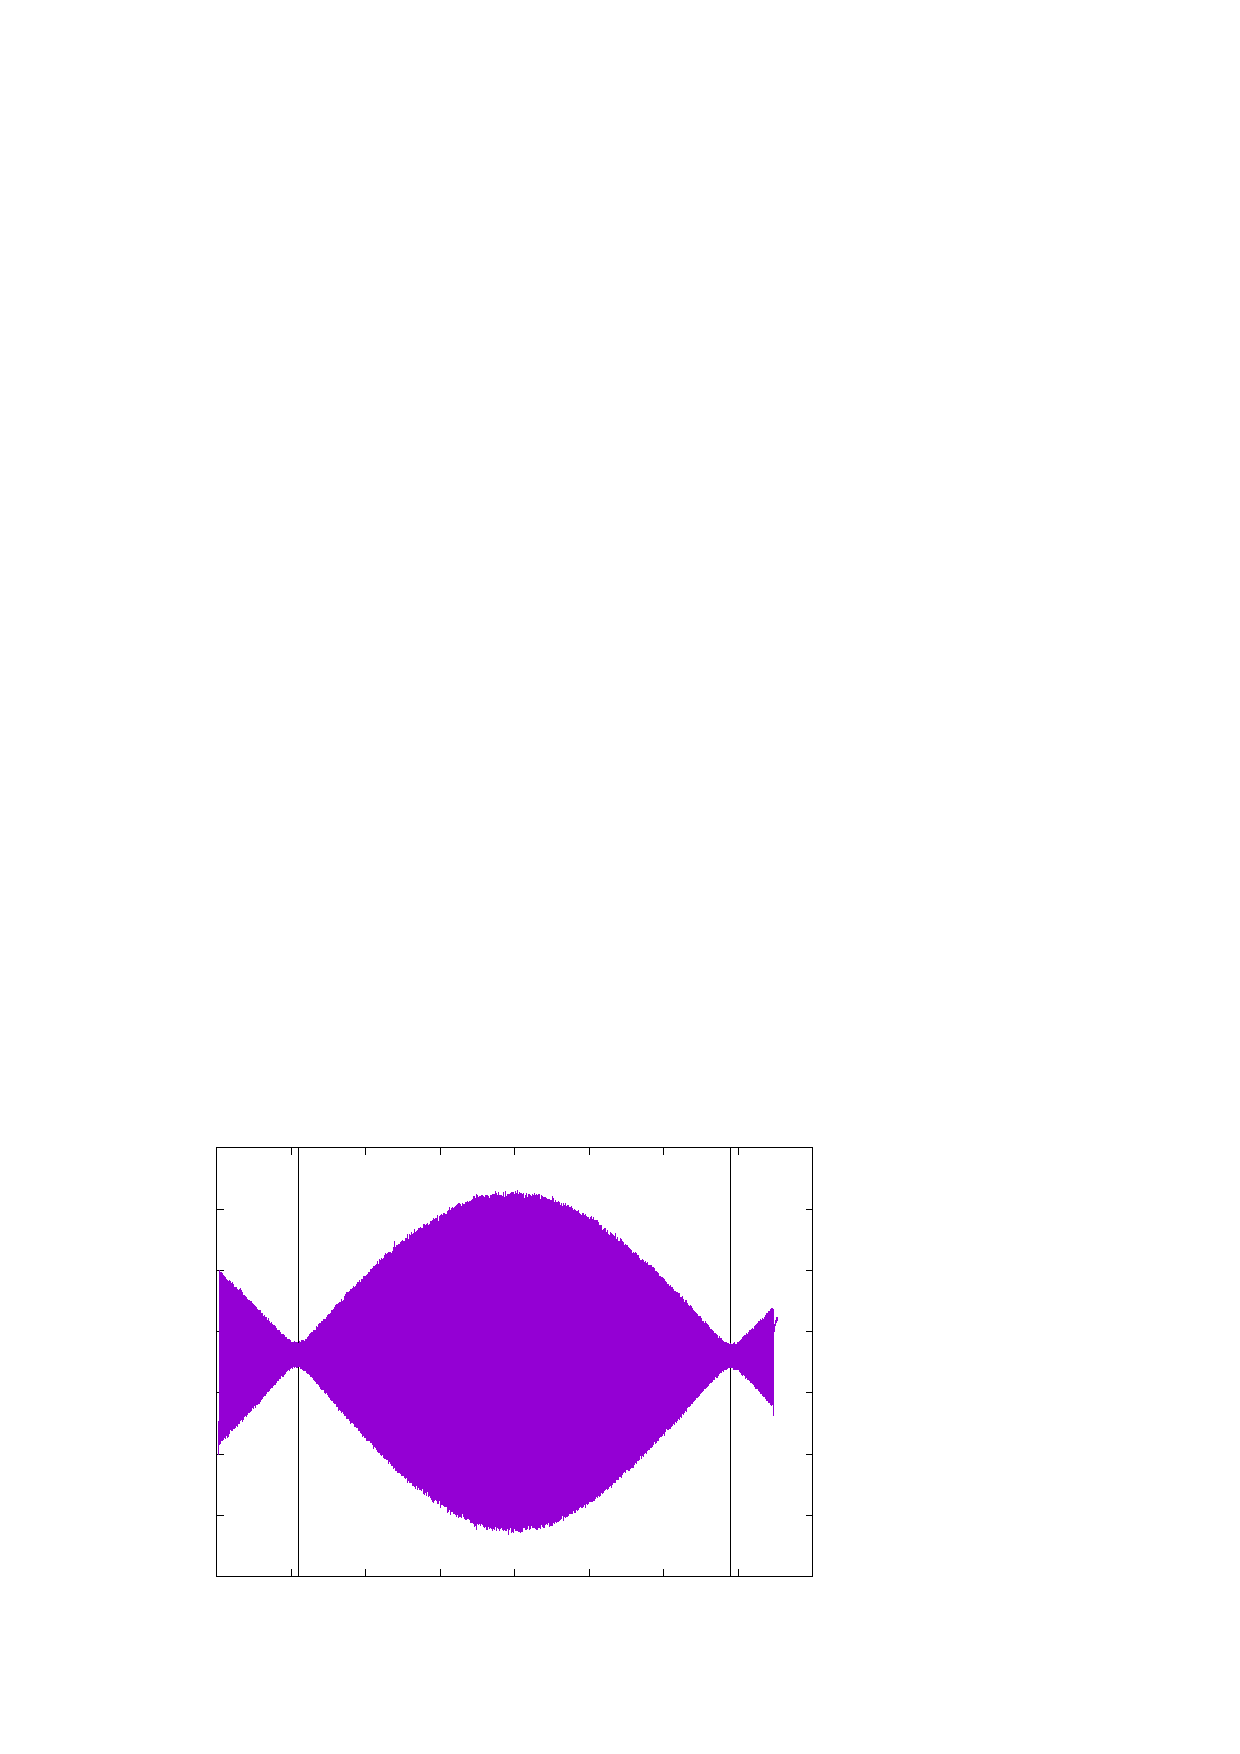
\includegraphics[width={360.00bp},height={252.00bp}]{Dominik/schwebung_na}}%
    \gplfronttext
  \end{picture}%
\endgroup
}
    \caption{Aufnahme der Schwebung des Interferogramms der Na-D Linie mit eingezeichneten Minima (Knoten)}
\end{figure}\\
Der Abstand zwischen zwei Knoten der Schwebung beträgt:
\begin{equation}
    \Delta S=\left(0,290\pm0,005\right)\,\text{mm}%8,295-8,005
\end{equation}
Dieser kann genutzt werden, um den Wellenlängenabstand der beiden Schwebungswellenlängen zu berechnen:%Minimas in der Schwebung werden erreicht für:
\begin{align}
    \cos\left(\Delta kl\right)&=0\\
    \Delta kl&=\frac{\left(2n-1\right)\pi}{2}\\
    \Delta k&=\frac{\left(2n-1\right)\pi}{2l}
\end{align}
Da wir einen 'Bauch' der Schwebung betrachten folgt: $l=S/2$ und $n=1$\\
Somit folgt für den Wellenlängenabstand der Schwebung im l-Raum:
\begin{align}
    \Delta k&=\frac{\pi}{S}\\
    \Delta \lambda&=\frac{\lambda_{Na}^2}{2S}\\
    \Delta \lambda&=\left(0,594\pm0,006\right)\,\text{nm}
\end{align}
Betrachten wir den Abstand zwischen den Literaturwerten für die Natrium D-1 und D-2 Linie $(\Delta\lambda=0,597\,\text{nm})$, so sehen wir, dass wir mit der Messung und dem Fehler diesen Wert einschließen.\\
Für die Amplitude einer Schwebung folgt aus den Fragen zur Vorbereitung:
\begin{equation}
    A=\sqrt{A_1^2+A_2^2+2A_1A_2\cos(\left|\omega_2-\omega_1\right|t)}
\end{equation}
Somit folgt für die Intensität im Knoten (Minima):
\begin{equation}
    A_K=\sqrt{A_1^2+A_2^2-2A_1A_2}=A_1-A_2
\end{equation}
Für die Intensität im Bauch (Maxima) folgt:
\begin{equation}
    A_B=A_1^2+A_2^2+2A_1A_2=A_1+A_2
\end{equation}
Wenn man nun das Intensitätsverhältnis/Amplitudenverhältnis $A_2/A_1$ haben möchte, kann man dies durch lösen des LGS bekommen:
\begin{equation}
    \frac{A_2}{A_1}=\frac{A_B-A_K}{A_B+A_K}
\end{equation}
Somit folgt für das gemessene Verhältnis (Ablesefehler: $0,001\,\text{V}$): %offset:0,325
\begin{equation}
    \frac{A_2}{A_1}=\left(0,875\pm0,002\right)%0,037_K/0,554_B
\end{equation}
Als Literaturwert wurde der Wert $0,8$ gefunden \citep[vgl.][S. 92]{Zusatzliteratur}.
Unser berechneter Wert schließt den theoretisch zu erwarteten Wert zwar nicht ein, liegt dennoch in dessen Größenordnung.
\subsection{Verbreiterungsmechanismus der Lampe}
Wie schon im vorherigen Teil zur Linienbreite gesagt wurde, ist die Natriumdampflampe doppelverbreitert.
Dies erkennt man daran, dass die Einhüllende des Interferogramms gaußförmig ist und nicht einer beidseitig abfallenden e-Funktion ähnelt.\\
Die Doppelverbreiterung kommt daher, dass die Lampe eine sehr hohe Betriebstemperatur von mehreren hundert Grad hat \citep[vgl.][]{Na-Dampf-Wiki}.
Durch die hohen Temperaturen dominiert die Doppelverbreiterung in Vergleich zur Druckverbreiterung.
\begin{figure}[h]
    \centering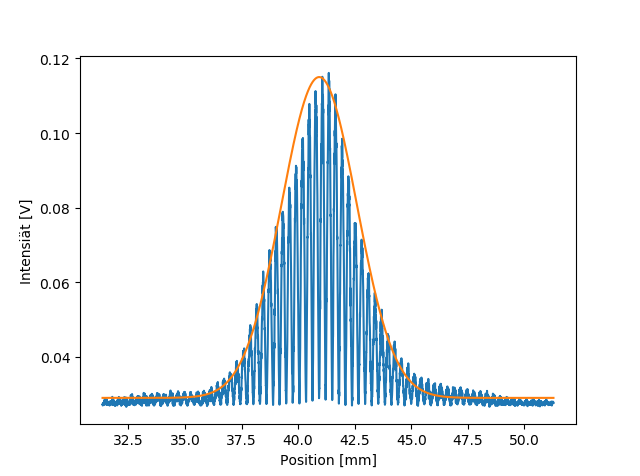
\includegraphics[width=0.8\textwidth]{Dominik/neu.png}
    \caption{Einhüllende des Interferogramms der Na-D Linie mit eingezeichnetem Gaußfit}
    \label{abbildung_ein}
\end{figure}
\newpage